% Created by tikzDevice version 0.6.2-92-0ad2792 on 2013-02-15 12:50:10
% !TEX encoding = UTF-8 Unicode
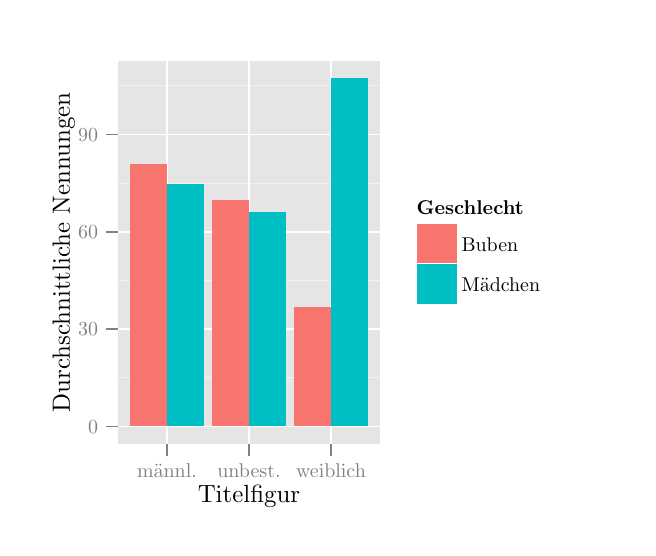
\begin{tikzpicture}[x=1pt,y=1pt]
\definecolor[named]{fillColor}{rgb}{1.00,1.00,1.00}
\path[use as bounding box,fill=fillColor,fill opacity=0.00] (0,0) rectangle (216.81,180.67);
\begin{scope}
\path[clip] (  0.00,  0.00) rectangle (216.81,180.67);
\definecolor[named]{drawColor}{rgb}{1.00,1.00,1.00}
\definecolor[named]{fillColor}{rgb}{1.00,1.00,1.00}

\path[draw=drawColor,line width= 0.6pt,line join=round,line cap=round,fill=fillColor] (  0.00,  0.00) rectangle (216.81,180.67);
\end{scope}
\begin{scope}
\path[clip] ( 32.55, 30.32) rectangle (127.38,168.63);
\definecolor[named]{fillColor}{rgb}{0.90,0.90,0.90}

\path[fill=fillColor] ( 32.55, 30.32) rectangle (127.38,168.63);
\definecolor[named]{drawColor}{rgb}{0.95,0.95,0.95}

\path[draw=drawColor,line width= 0.3pt,line join=round] ( 32.55, 54.18) --
	(127.38, 54.18);

\path[draw=drawColor,line width= 0.3pt,line join=round] ( 32.55, 89.34) --
	(127.38, 89.34);

\path[draw=drawColor,line width= 0.3pt,line join=round] ( 32.55,124.50) --
	(127.38,124.50);

\path[draw=drawColor,line width= 0.3pt,line join=round] ( 32.55,159.66) --
	(127.38,159.66);
\definecolor[named]{drawColor}{rgb}{1.00,1.00,1.00}

\path[draw=drawColor,line width= 0.6pt,line join=round] ( 32.55, 36.60) --
	(127.38, 36.60);

\path[draw=drawColor,line width= 0.6pt,line join=round] ( 32.55, 71.76) --
	(127.38, 71.76);

\path[draw=drawColor,line width= 0.6pt,line join=round] ( 32.55,106.92) --
	(127.38,106.92);

\path[draw=drawColor,line width= 0.6pt,line join=round] ( 32.55,142.08) --
	(127.38,142.08);

\path[draw=drawColor,line width= 0.6pt,line join=round] ( 50.33, 30.32) --
	( 50.33,168.63);

\path[draw=drawColor,line width= 0.6pt,line join=round] ( 79.97, 30.32) --
	( 79.97,168.63);

\path[draw=drawColor,line width= 0.6pt,line join=round] (109.60, 30.32) --
	(109.60,168.63);
\definecolor[named]{fillColor}{rgb}{0.97,0.46,0.43}

\path[fill=fillColor] ( 37.00, 36.60) rectangle ( 50.33,131.36);
\definecolor[named]{fillColor}{rgb}{0.00,0.75,0.77}

\path[fill=fillColor] ( 50.33, 36.60) rectangle ( 63.67,124.32);
\definecolor[named]{fillColor}{rgb}{0.97,0.46,0.43}

\path[fill=fillColor] ( 66.63, 36.60) rectangle ( 79.97,118.29);
\definecolor[named]{fillColor}{rgb}{0.00,0.75,0.77}

\path[fill=fillColor] ( 79.97, 36.60) rectangle ( 93.30,113.96);
\definecolor[named]{fillColor}{rgb}{0.97,0.46,0.43}

\path[fill=fillColor] ( 96.27, 36.60) rectangle (109.60, 79.63);
\definecolor[named]{fillColor}{rgb}{0.00,0.75,0.77}

\path[fill=fillColor] (109.60, 36.60) rectangle (122.94,162.34);
\end{scope}
\begin{scope}
\path[clip] (  0.00,  0.00) rectangle (216.81,180.67);
\definecolor[named]{drawColor}{rgb}{0.50,0.50,0.50}

\node[text=drawColor,anchor=base east,inner sep=0pt, outer sep=0pt, scale=  0.72] at ( 25.44, 34.12) {0};

\node[text=drawColor,anchor=base east,inner sep=0pt, outer sep=0pt, scale=  0.72] at ( 25.44, 69.28) {30};

\node[text=drawColor,anchor=base east,inner sep=0pt, outer sep=0pt, scale=  0.72] at ( 25.44,104.44) {60};

\node[text=drawColor,anchor=base east,inner sep=0pt, outer sep=0pt, scale=  0.72] at ( 25.44,139.60) {90};
\end{scope}
\begin{scope}
\path[clip] (  0.00,  0.00) rectangle (216.81,180.67);
\definecolor[named]{drawColor}{rgb}{0.50,0.50,0.50}

\path[draw=drawColor,line width= 0.6pt,line join=round] ( 28.29, 36.60) --
	( 32.55, 36.60);

\path[draw=drawColor,line width= 0.6pt,line join=round] ( 28.29, 71.76) --
	( 32.55, 71.76);

\path[draw=drawColor,line width= 0.6pt,line join=round] ( 28.29,106.92) --
	( 32.55,106.92);

\path[draw=drawColor,line width= 0.6pt,line join=round] ( 28.29,142.08) --
	( 32.55,142.08);
\end{scope}
\begin{scope}
\path[clip] (  0.00,  0.00) rectangle (216.81,180.67);
\definecolor[named]{drawColor}{rgb}{0.50,0.50,0.50}

\path[draw=drawColor,line width= 0.6pt,line join=round] ( 50.33, 26.05) --
	( 50.33, 30.32);

\path[draw=drawColor,line width= 0.6pt,line join=round] ( 79.97, 26.05) --
	( 79.97, 30.32);

\path[draw=drawColor,line width= 0.6pt,line join=round] (109.60, 26.05) --
	(109.60, 30.32);
\end{scope}
\begin{scope}
\path[clip] (  0.00,  0.00) rectangle (216.81,180.67);
\definecolor[named]{drawColor}{rgb}{0.50,0.50,0.50}

\node[text=drawColor,anchor=base,inner sep=0pt, outer sep=0pt, scale=  0.72] at ( 50.33, 18.24) {männl.};

\node[text=drawColor,anchor=base,inner sep=0pt, outer sep=0pt, scale=  0.72] at ( 79.97, 18.24) {unbest.};

\node[text=drawColor,anchor=base,inner sep=0pt, outer sep=0pt, scale=  0.72] at (109.60, 18.24) {weiblich};
\end{scope}
\begin{scope}
\path[clip] (  0.00,  0.00) rectangle (216.81,180.67);
\definecolor[named]{drawColor}{rgb}{0.00,0.00,0.00}

\node[text=drawColor,anchor=base,inner sep=0pt, outer sep=0pt, scale=  0.90] at ( 79.97,  9.03) {Titelfigur};
\end{scope}
\begin{scope}
\path[clip] (  0.00,  0.00) rectangle (216.81,180.67);
\definecolor[named]{drawColor}{rgb}{0.00,0.00,0.00}

\node[text=drawColor,rotate= 90.00,anchor=base,inner sep=0pt, outer sep=0pt, scale=  0.90] at ( 15.23, 99.47) {Durchschnittliche Nennungen};
\end{scope}
\begin{scope}
\path[clip] (  0.00,  0.00) rectangle (216.81,180.67);
\definecolor[named]{fillColor}{rgb}{1.00,1.00,1.00}

\path[fill=fillColor] (136.25, 76.46) rectangle (195.90,122.49);
\end{scope}
\begin{scope}
\path[clip] (  0.00,  0.00) rectangle (216.81,180.67);
\definecolor[named]{drawColor}{rgb}{0.00,0.00,0.00}

\node[text=drawColor,anchor=base west,inner sep=0pt, outer sep=0pt, scale=  0.72] at (140.52,113.25) {\bfseries Geschlecht};
\end{scope}
\begin{scope}
\path[clip] (  0.00,  0.00) rectangle (216.81,180.67);
\definecolor[named]{drawColor}{rgb}{1.00,1.00,1.00}
\definecolor[named]{fillColor}{rgb}{0.95,0.95,0.95}

\path[draw=drawColor,line width= 0.6pt,line join=round,line cap=round,fill=fillColor] (140.52, 95.18) rectangle (154.97,109.64);
\end{scope}
\begin{scope}
\path[clip] (  0.00,  0.00) rectangle (216.81,180.67);
\definecolor[named]{fillColor}{rgb}{0.97,0.46,0.43}

\path[fill=fillColor] (140.52, 95.18) rectangle (154.97,109.64);

\path[] (140.52, 95.18) --
	(154.97,109.64);
\end{scope}
\begin{scope}
\path[clip] (  0.00,  0.00) rectangle (216.81,180.67);
\definecolor[named]{drawColor}{rgb}{1.00,1.00,1.00}
\definecolor[named]{fillColor}{rgb}{0.95,0.95,0.95}

\path[draw=drawColor,line width= 0.6pt,line join=round,line cap=round,fill=fillColor] (140.52, 80.73) rectangle (154.97, 95.18);
\end{scope}
\begin{scope}
\path[clip] (  0.00,  0.00) rectangle (216.81,180.67);
\definecolor[named]{fillColor}{rgb}{0.00,0.75,0.77}

\path[fill=fillColor] (140.52, 80.73) rectangle (154.97, 95.18);

\path[] (140.52, 80.73) --
	(154.97, 95.18);
\end{scope}
\begin{scope}
\path[clip] (  0.00,  0.00) rectangle (216.81,180.67);
\definecolor[named]{drawColor}{rgb}{0.00,0.00,0.00}

\node[text=drawColor,anchor=base west,inner sep=0pt, outer sep=0pt, scale=  0.72] at (156.78, 99.93) {Buben};
\end{scope}
\begin{scope}
\path[clip] (  0.00,  0.00) rectangle (216.81,180.67);
\definecolor[named]{drawColor}{rgb}{0.00,0.00,0.00}

\node[text=drawColor,anchor=base west,inner sep=0pt, outer sep=0pt, scale=  0.72] at (156.78, 85.48) {Mädchen};
\end{scope}
\end{tikzpicture}
